\section{Intermediate Representations}
\begin{figure*}
  \centering
  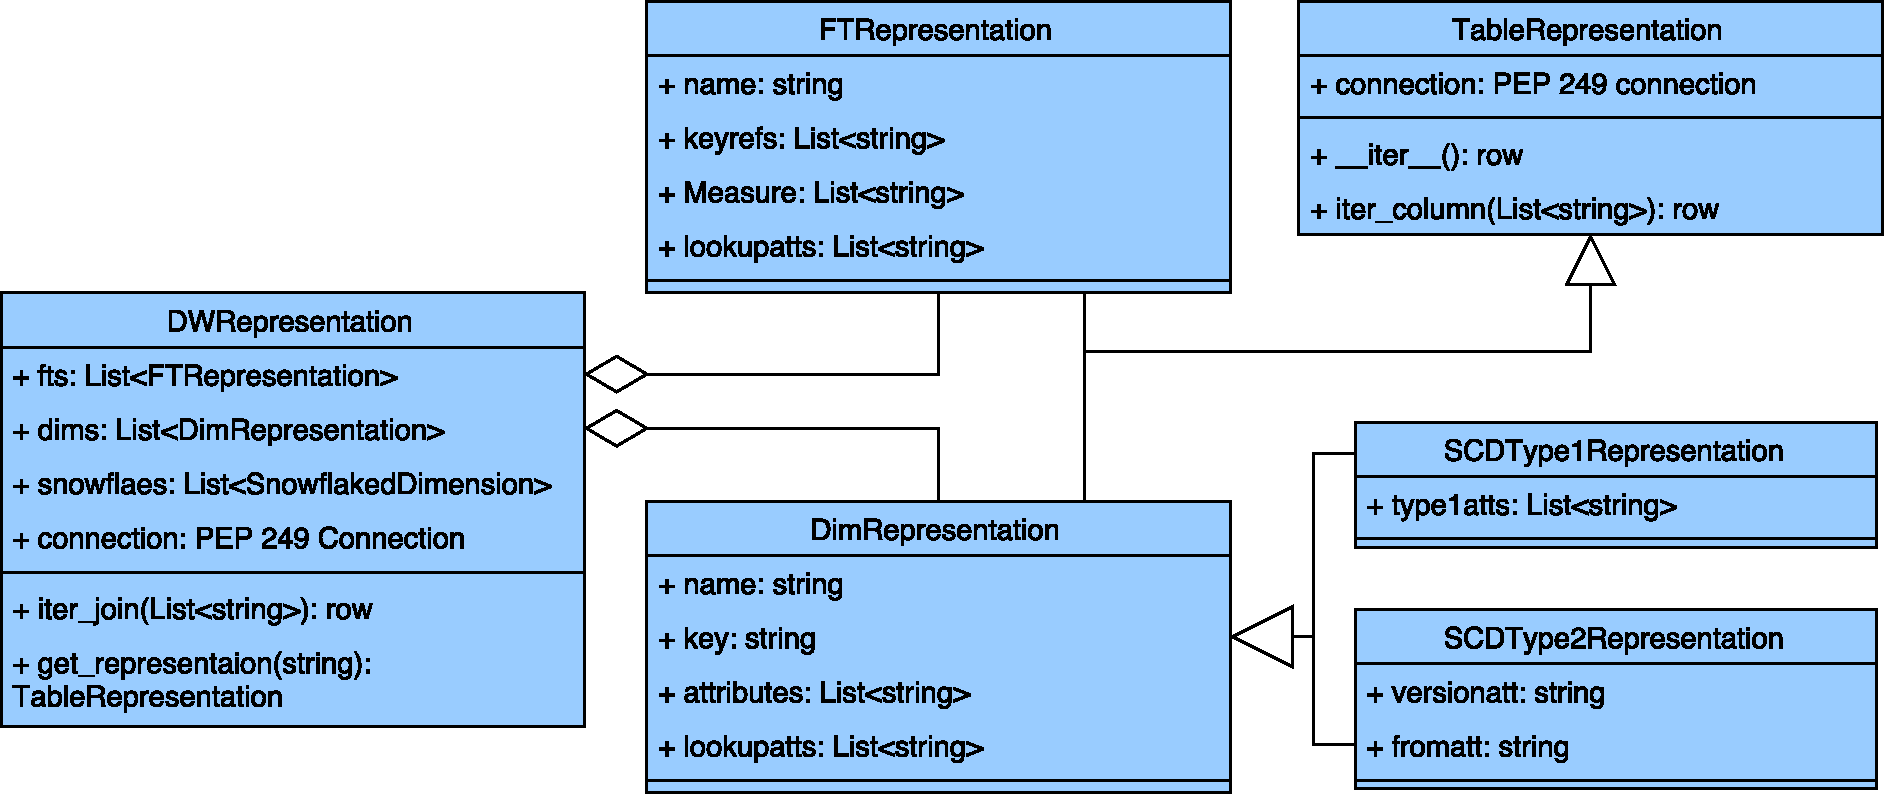
\includegraphics[width=0.7\textwidth]{figures/dwrep_uml.pdf}
  \caption{UML diagram of the intermediate representations}
  \label{fig:dwrep}
\end{figure*}

This section will go into details about the different intermediate representations that we use in the predicates. These representations are used as a way of giving a standardized input to the predicates, that allow for easy access to the DW. There are two main forms of intermediate representations, the \textit{DWRepresentation} and the \textit{TableRepresentation}. Where the DWRepresentation represents the DW as a whole, and the TableRepresentation has a lot of subclasses representing different kinds of tables. A UML diagram of the intermediate representations can be seen in \cref{fig:dwrep}.

\subsection{DWRepresentation}
The \textit{DWRepresentation} is a container object, containing information about the DW schema. It also provides methods of connecting to, and extracting data from, the DW. It is created by the \textit{RepresentationMaker} by aggregating a number of \textit{TableRepresentations}, and is used as link to the DW that future predicates can use.

The DWRepresentation contains information regarding the following,

\begin{description}
\item[Dimensions] Contains a list of \textit{DimRepresentations}, detailing each dimension in the DW. Different kind of dimensions are supported here, e.g. slowly changing dimensions.
\item[FactTables] Contains a list of FactTables in the DW.
\item[Snowflakes] Contains a list of Snowflaked dimensions, this is used to find the structure of the DW.
\item[Connection] A connection to the DW, so that we may query it for data later on.
\end{description} 
 
Besides containing the previously mentioned information, the DW also provides some functionality for accessing the data contained in the DW. It does this in one of two ways, you can request for a specific \textit{TableRepresentation} by providing a table name. Or you can iterate over a natural join of tables. This is especially useful for when constructing predicates that you could imagine should work on a join of tables.

\subsection{TableRepresentation}
\textit{TableRepresentation} is a superclass used for retrieving data from specific tables. Instatations of its subclasses contains additional information regarding the tables themselves, such as the table name, attributes and et cetera. These are created by extracting information regarding the tables from the scope of the executed pygrametl program. Specifically from table objects there. 

The currently supported tables are,

\begin{itemize}
\item Dimension
\item Type 1 Slowly Changing Dimensions
\item Type 2 Slowly Changing Dimensions
\item FactTables
\end{itemize}

The data within the specific table can be accesed by iterating over the TableRepresentation. This queries the DW and yields a single row at a time.
